\chapter{Human simulated performance testing (HSUP)}
\label{sec:HSUP}

Human simulated performance (HSUP) testing is used to measure the performance of smart devices in human-like operation. It uses high-speed camera to track visual changes in the display while the device is operated by a robot.

HSUP consists of three distinct measurement / analysis types: Watchdog, scroll performance analysis (SPA) and pen-to-ink (P2I) analysis. These are described in more detail in sections below.

\begin{figure}[!h]
	\centering
	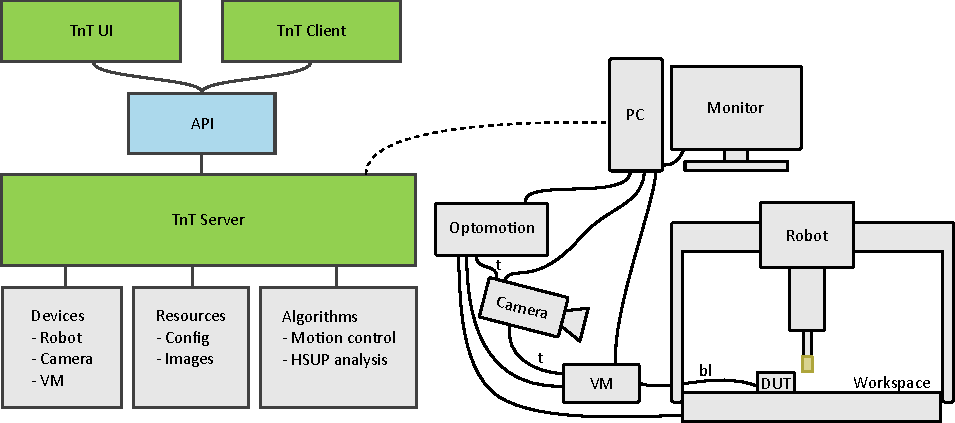
\includegraphics{hsup_sw}
	\caption{HSUP software components and hardware. Trigger signals are denoted by \texttt{t} and backlight synchronization signal is denoted by \texttt{bl}. The boxes under TnT Server denote the parts in server that are relevant for HSUP.}
	\label{fig:hsup_sw}
\end{figure}

The software components and hardware setup is illustrated in Figure \ref{fig:hsup_sw}. In HSUP, an external high speed camera is used to track changes on the DUT when robot performs some gesture. TnT Client or TnT UI are used to request an HSUP measurement and analysis. TnT server then commands the robot to perform the motion and collects any images received from the camera. The images are analyzed and stored to image database on the disk and the analysis results are stored to memory. The results can then be obtained from the server as a separate request once the measurement and analysis are complete. It is also possible to request server to analyze the stored images later.

TnT UI provides an HSUP page to set various camera parameters and quickly test the measurements. To get the measurements to work correctly for the first time, some amount of experimentation with the parameters is usually required. The obtained parameters can be saved to a configuration file and used later in scripts via TnT Client. The HSUP page cannot currently be used to command robot movements for HSUP measurements. Instead user must use TnT Client or the Sequence generator page to specify the required movements.

In HSUP the camera capture process is not triggered by software but instead direct hardware triggering is used to get exact timing between motion and image capture. There are two alternative ways to implement the triggering based on whether also synchronization to DUT backlight is required: 1) No backlight synchronization. Optomotion triggers the camera based on voice coil axis encoder change. 2) Backlight synchronization is required. OptoFidelity proprietary Video Multimeter (VM) is used to trigger the camera. Triggering is based on signal from voice coil encoder and a backlight sensor that is attached to the DUT screen. TnT Server is connected also to VM to set triggering parameters.

\section{HSUP in TnT UI}

HSUP measurement and analysis can be performed using TnT UI. It has "HSUP" page which contains controls for each measurement type as shown in Figure \ref{fig:ui_hsup}.

\begin{figure}[h]
	\centering
	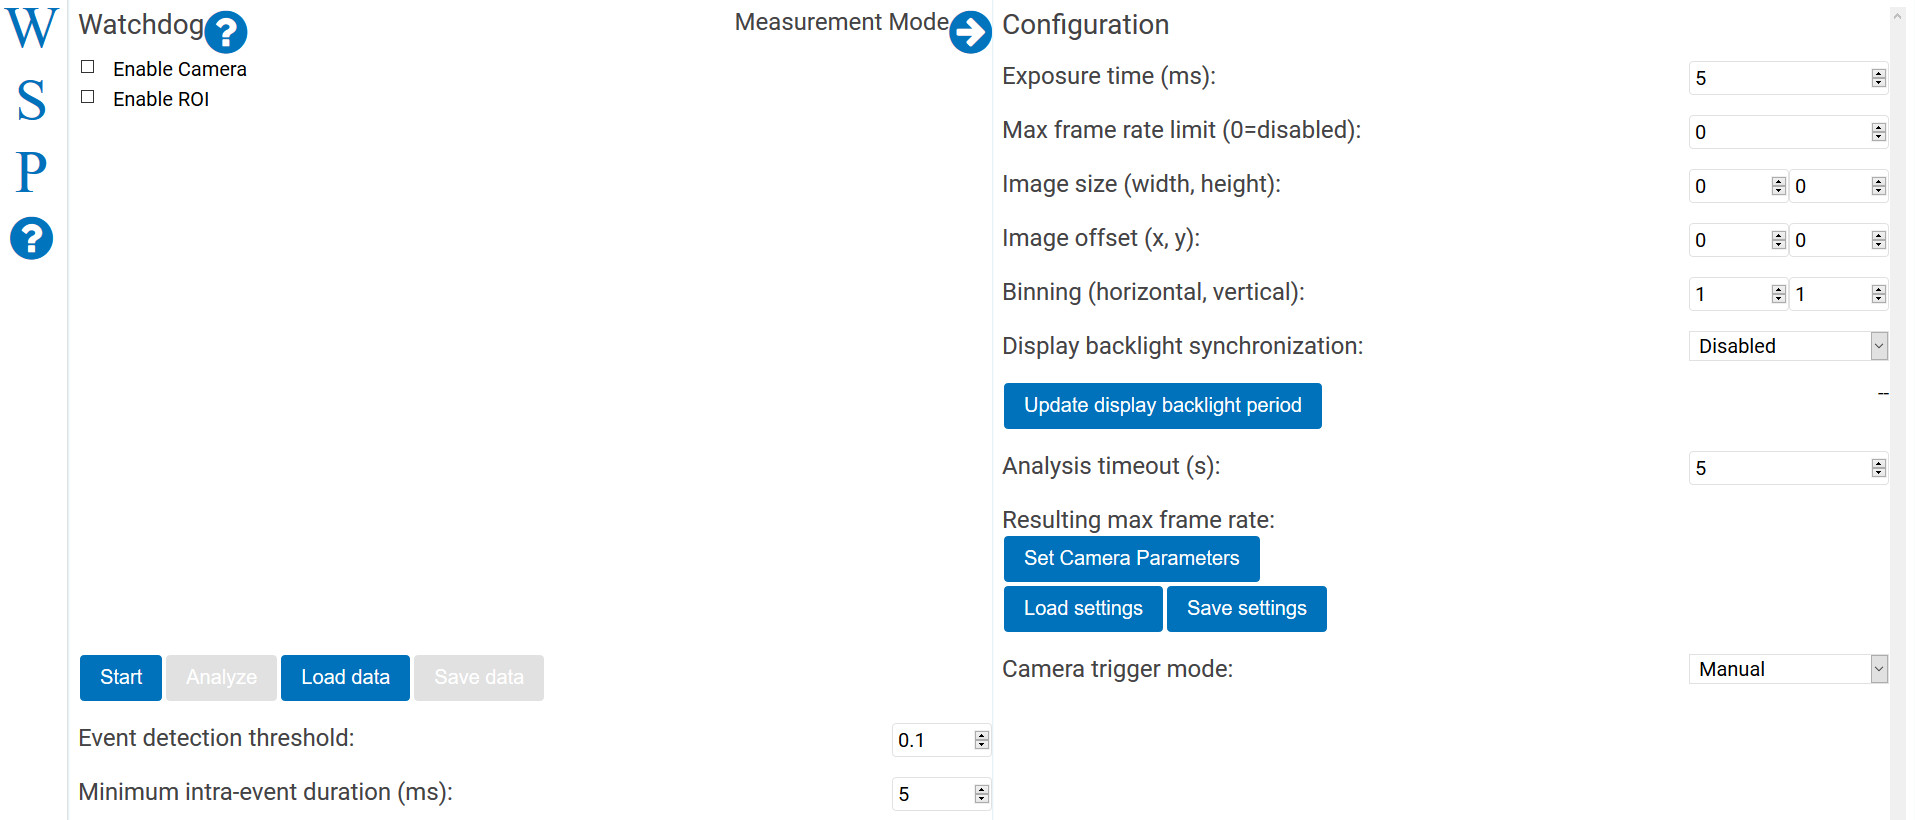
\includegraphics[width=0.9\linewidth]{ui_hsup.jpg}
	\caption{HSUP page in TnT UI.}
	\label{fig:ui_hsup}
\end{figure}

\input{from_ui_repo/hsup_common}

\input{from_ui_repo/hsup_watchdog}

\input{from_ui_repo/hsup_spa}

\input{from_ui_repo/hsup_p2i}

\section{HSUP via TnT Client}

HSUP measurements and analysis can also be run from Python scripts by use of TnT Client. See the TnT Client API reference guide for more details and the example script in the client Python package.

\importantbox{If you are using HSUP via Client, make sure that the HSUP camera is not open in TnT UI. Having the camera open in more than one instance might interfere with script execution.}